There is a significant improvement in how quickly the image converges to something that looks like the number in question. We can assume that this is because there is much less variance in how the number itself is written. When writing a 1, there are much fewer variations such as a horizontal line through the middle, like in the sevens. This means that it will converge to something useful more quickly.\\
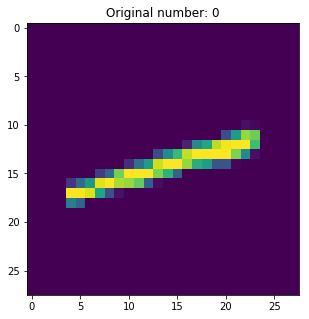
\includegraphics[width=0.25\linewidth]{1orig0.png}\\
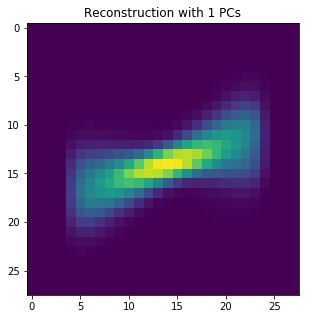
\includegraphics[width=0.25\linewidth]{1rec01.png}
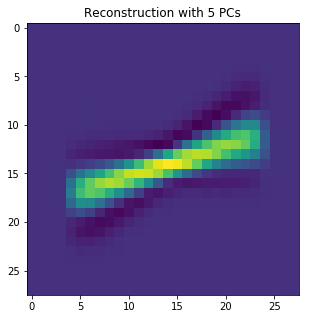
\includegraphics[width=0.25\linewidth]{1rec05.png}
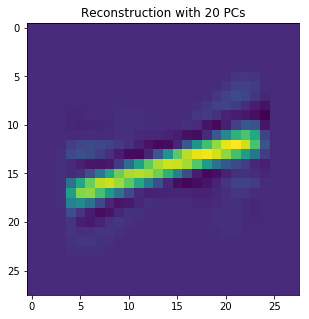
\includegraphics[width=0.25\linewidth]{1rec020.png}
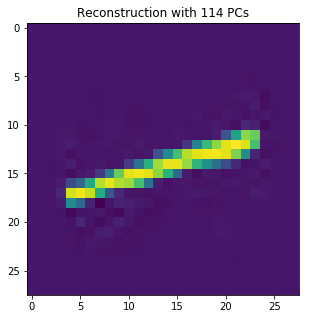
\includegraphics[width=0.25\linewidth]{1rec0114.png}\\
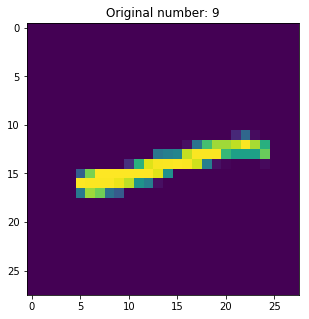
\includegraphics[width=0.25\linewidth]{1orig9.png}\\
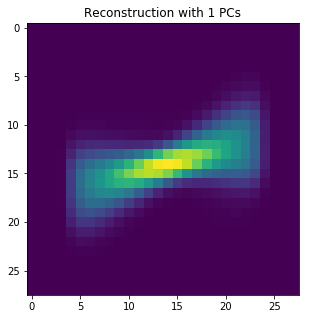
\includegraphics[width=0.25\linewidth]{1rec91.png}
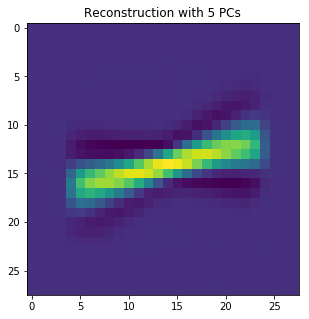
\includegraphics[width=0.25\linewidth]{1rec95.png}
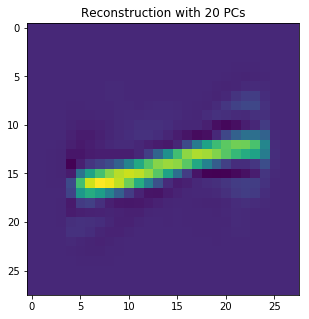
\includegraphics[width=0.25\linewidth]{1rec920.png}
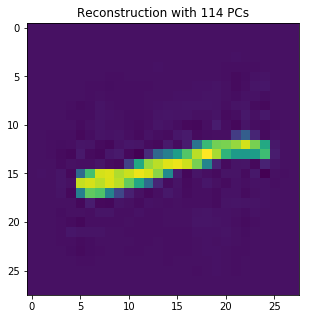
\includegraphics[width=0.25\linewidth]{1rec9114.png}\\